\documentclass[12pt]{article}
\usepackage{graphicx}
\usepackage{svg}
\usepackage{blindtext}
\usepackage[abspath]{currfile}


% \graphicspath{{img/}} % set the root directory name containing images


\begin{document}


\section{First section}

\blindtext[1]
% \includegraphics{universe} % the best practice is to omit the file extension because it will prompt LaTeX to search for all the supported formats
% \includegraphics{universe.jpg}
% \includegraphics[width=5cm]{universe.jpg}
\includegraphics[width=5cm]{\currfileabsdir/img/universe.jpg}
\blindtext[1]

\vspace{8mm}

\blindtext[1]

% \includesvg[width=\textwidth]{vietnam_flag}
% \includesvg[width=8cm]{vietnam_flag}
\includesvg[width=8cm]{\currfileabsdir/img/vietnam_flag}

\blindtext[1]



% \includegraphics[width=..., height=..., scale=0.5, keepaspectratio]{\currfileabsdir/img/universe.jpg}
% \includegraphics[width=0.7\textwidth,angle=90]{\currfileabsdir/img/universe.jpg}



\end{document}
